\chapter{FeynCalc and FeynArt}
\lstset{backgroundcolor=\color{solarized-base02}, frame=single, rulecolor=\color{solarized-base01}, framexleftmargin=0.5ex, xleftmargin=0.3ex, numbers=none}
\textit{FeynCalc} and \textit{FeynArt} are \textit{Mathematica} packages for doing QFT computations.
I don't know these packages very well but this appendix compiles some of the parts that I've found useful in this course.

To start the file use
\begin{lstlisting}[language=mathematica, gobble=4]
    $LoadAddOns = {"FeynArts"};
    Get["FeynCalc`"]
\end{lstlisting}

\section{Basics}
A four-vector, such as \(p^\mu\), is represented in \textit{FeynCalc} as one of the following
\begin{lstlisting}[language=mathematica, gobble=4, mathescape]
    FourVector[p, $\mu$]
    FV[p, $\mu$]
\end{lstlisting}
This gives \(p^\mu\), all indices are up in \textit{FeynCalc}, which is fine as long as we keep it in mind when converting from \textit{FeynCalc} results to normal notation.
The product \(p^\mu q_\mu\) is represented by one of the following
\begin{lstlisting}[language=mathematica, gobble=4, mathescape]
    FV[p, $\mu$] FV[q, $\mu$] // Contract
    ScalarProduct[p, q]
    SP[p, q]
\end{lstlisting}
We can also use the shorthand £SP[p]£ to get \(p^2\).
We can assign values to scalar products, for example, if we have \(p\) as the momentum of an on-shell particle of mass \(m\) we may wish to define
\begin{lstlisting}[language=mathematica, gobble=4, mathescape]
    ScalarProduct[p, p] = m$\,{}^2$
\end{lstlisting}
Then evaluating £SP[p]£ will give \(m^2\).

The derivative is given using
\begin{lstlisting}[language=mathematica, gobble=4, mathescape]
    FourDivergence[expr, FV[x, $\mu$]]
\end{lstlisting}
to compute the derivative of £expr£ with respect to \(x^\mu\).
Similarly the d'Alembert operator is implemented as
\begin{lstlisting}[language=mathematica, gobble=4, mathescape]
    FourLaplacian[expr, p, p]
\end{lstlisting}
to compute the d'Alembert acting on £expr£ in momentum space.
For example,
\begin{lstlisting}[language=mathematica, gobble=4, mathescape]
    FourDivergence[Exp[-$\mathbb{i}$SP[p,x]], FV[p,$\mu$]]
    FourLaplacian[Exp[-$\mathbb{i}$SP[p,x]], x, x]
\end{lstlisting}
gives
\begin{equation}
    -ip^\mu \e^{-ip\cdot x}, \qqand -p^2 \e^{-ip\cdot x}
\end{equation}
respectively.

\section{Gamma Matrices}
The gamma matrices are given by
\begin{lstlisting}[language=mathematica, gobble=4, mathescape]
    GA[$\mu$]
\end{lstlisting}
Slash notation can be done using
\begin{lstlisting}[language=mathematica, gobble=4, mathescape]
    GS[p]
\end{lstlisting}
to produce \(\slashed{p}\), although this is then written as \(\gamma \cdot p\).
Note that since the gamma matrices don't commute when doing products with them we need to use £.£ (£Dot£) as the product, instead of the default product (£Times£) which is assumed to commute.

The command £DiracOrder£ places a product of gamma matrices in a canonical order, for example the following
\begin{lstlisting}[language=mathematica, gobble=4, mathescape]
    GA[$\mu$].GA[$\nu$] // DiracOrder
    GA[$\nu$].GA[$\mu$] // DiracOrder
\end{lstlisting}
gives
\begin{equation}
    \gamma^\mu\gamma^\nu, \qqand 2g^{\mu\nu} - \gamma^\mu\gamma^\nu
\end{equation}
respectively, which are equivalent to the initial expressions and use the anticommutation relations to reorder products of gamma matrices.

Terms involving gamma matrices can be simplified using £DiracSimplify£, for example,
\begin{lstlisting}[language=mathematica, gobble=4, mathescape]
    GA[$\mu$].GA[$\mu$] // DiracSimplify
    GA[$\mu$].GS[a].GA[$\mu$] // DiracSimplify
    GA[$\mu$].GS[a].GS[b].GS[c].GS[d].GA[$\mu$] // DiracSimplify
\end{lstlisting}
give
\begin{equation}
    4, \qquad -2\slashed{p}, \qqand 2(\slashed{d}\slashed{a}\slashed{b}\slashed{c} + \slashed{c}\slashed{b}\slashed{a}\slashed{d})
\end{equation}
respectively.

\section{FeynArt}
\textit{FeynArt} is a package for creating Feynman diagrams.
The first command we'll need is
\begin{lstlisting}[language=mathematica, gobble=4]
    InsertFields[CreateTopologies[...],
        {incoming particles} -> {outgoing paritlces}
    ]
\end{lstlisting}
Here
\begin{lstlisting}[language=mathematica, gobble=4]
    CreateTopologies[l, i -> o]
\end{lstlisting}
tells \textit{FeynArt} to generate all diagrams with \(i\) incoming particles, \(o\) outgoing particles, and \(l\) loops.
We then list the incoming and outgoing particles for £InsertFields£.
A fermion is represented by £F£ with some argument.
The first argument of £F£ is an integer from 1 to 4, these represent generic neutrinos, massive leptons, up-type quarks, and down-type quarks, in that order.
The second argument is a list of integers.
The simplest case being a list of one integer from 1 to 3, which tells us the generation.
So, for example, an electron is £F[2, {1}]£ and a charm quark is £F[3, {2}]£.
The antiparticle is then given by £-F[...]£, so £-F[2, {1}]£ is a positron and £F[1, {3}]£ is an antitau neutrino.

There are two arguments to £InsertFields£ that we'll use, one is \lstinline[style=mathematica, breaklines]|InsertionLevel -> {Classes}|.
This is related to how different levels of generality are implemented in \textit{FeynArt}.
The second is £Restrictions -> QEDOnly£, which tells \textit{FeynArt} to ignore any processes that aren't QED.

Finally, we need
\begin{lstlisting}[language=mathematica, gobble=4]
    CreateFeynAmp[...]
\end{lstlisting}
which takes the result of £InsertFields£ and creates a list of corresponding Feynman amplitudes.

\section{\texorpdfstring{\(\Pe\APe \to \Pmu\APmu\)}{Electron-Positron to Muon-Antimuon}}
\label{sec:electron-positron to muon-antimuon with feyncalc}
In \cref{chap:electron-positron to muon-antimuon} we computed the leading order QED contribution to the \(\Pe\APe \to \Pmu\APmu\) process.
Here we do the same calculation using \textit{FeynCalc} and \textit{FeynArt}.
First, define the interaction:
\begin{lstlisting}[language=mathematica, gobble=4]
    feynmanDiagram = InsertFields[
        CreateTopologies[0, 2 -> 2],
        {F[2, {1}], -F[2, {1}]} -> {F[2, {2}], -F[2, {2}]},
        InsertionLevel -> {Classes},
        Restrictions -> QEDOnly
    ]
\end{lstlisting}
We can print the diagram with the following command:
\begin{lstlisting}[language=mathematica, gobble=4]
    Paint[feynmanDiagram,
        ColumnsXRows -> {1, 1}, Numbering -> Simple,
        SheetHeader -> None, ImageSize -> {256, 256}
    ]
\end{lstlisting}
This produces the diagram shown in \cref{fig:feynart result}.

\begin{figure}
    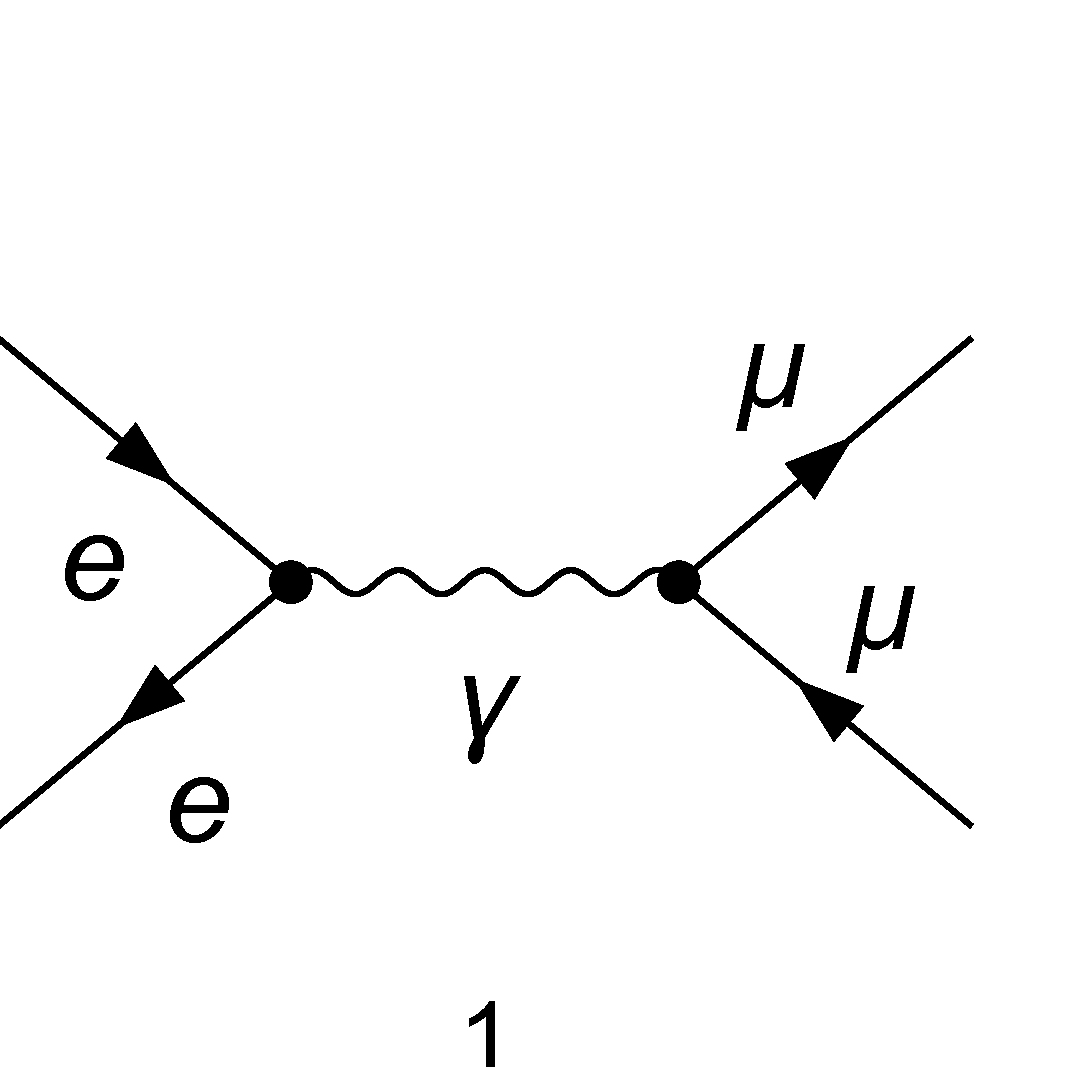
\includegraphics[width=0.8\textwidth]{images/feynart-fd-ee-mumu}
    \caption{The Feynman diagram generated by \textit{FeynArt}.}
    \label{fig:feynart result}
\end{figure}

We can turn this into the amplitude as follows:
\begin{lstlisting}[language=mathematica, gobble=4]
    amp[0] = FCFAConvert[CreateFeynAmp[diags],
        IncomingMomenta -> {p1, p2},
        OutgoingMomenta -> {p3, p4},
        UndoChiralSplittings -> True,
        ChangeDimension -> 4, List -> False, 
        SMP -> True, Contract -> True
    ]
\end{lstlisting}
here we use the \textit{FeynArt} function £CreateFeynAmp£ to create the Feynman amplitude and then the £FeynCalc£ function £FCFAConvert£ to turn the amplitude into a \textit{FeynCalc} compatible result.
This sets the momenta of the particles and does some simplifications.

Next we run £FCClearScalarProducts[]£ which just clears any defined values of scalar products, and is good practice to run at the start of each new calculation.
We can run the following commands:
\begin{lstlisting}[language=mathematica, gobble=4]
    MakeBoxes[p1, TraditionalForm] :=
        "\!\(\*SubscriptBox[\(p\),\(1\)]\)";
    MakeBoxes[p2, TraditionalForm] :=
        "\!\(\*SubscriptBox[\(p\),\(2\)]\)";
    MakeBoxes[p3, TraditionalForm] :=
        "\!\(\*SubscriptBox[\(p\),\(3\)]\)";
    MakeBoxes[p4, TraditionalForm] :=
        "\!\(\*SubscriptBox[\(p\),\(4\)]\)";
\end{lstlisting}
which just tell \textit{Mathematica} to pretty print £p1£ as \(p_1\) and so on.

Then we can run
\begin{lstlisting}[language=mathematica, gobble=4]
    SetMandelstam[s, t, u, p1, p2, -p3, -p4,
        SMP["m_e"], SMP["m_e"], SMP["m_mu"], SMP["m_mu"]]
\end{lstlisting}
The command
\begin{lstlisting}[language=mathematica, gobble=4]
    SetMandelstam[s, t, u, p1, p2, p3, p4,
        m1, m2, m3, m4]
\end{lstlisting}
sets the Mandelstam variables \(s = (p_1 + p_2)^2\), \(t = (p_1 + p_3)^2\), and \(u = (p_1 + p_4)^2\).
It also sets \(p_i^2 = m_i^2\).
Note that £SMP["par"]£ displays a parameter to the standard model, such as the mass of an electron, in a standard way.

Next we compute the amplitude squared:
\begin{lstlisting}[language=mathematica, gobble=4]
    ampSquared[0] = Simplify[DiracSimplify[
        (FermionSpinSum[#1, ExtraFactor -> 1/4] &)
        [FeynAmpDenominatorExplicit[amp[0]
        *ComplexConjugate[amp[0]]]]
    ]]
\end{lstlisting}
This squares the amplitude, computing \(\amplitude \amplitude^*\), then sums over the helicities with £FermionSpinSum£, manually including the factor of \(1/4\) from averaging over initial helicity states.
We then use \textit{FeynCalc}'s £DiracSimplify£ to simplify the spinor part and then \textit{Mathematica}'s £Simplify£ to simplify the normal algebra.
The result is
\begin{equation*}
    \frac{8e^4[m_{\symrm{e}}^2(p_3 \cdot p_4) + m_{\text{μ}}^2(p_1 \cdot p_2) + (p_1 \cdot p_4)(p_2 \cdot p3) + (p_1\cdot p_3)(p_2 \cdot p_4) + 2m_{\symrm{e}}^2m_{\text{μ}}^2]}{[2(p_3 \cdot p_4) + p_3^2 + p_4^2]^2}.
\end{equation*}

Now we make the approximation that the particle masses are negligible, which we do through
\begin{lstlisting}[language=mathematica, gobble=4]
    ampSquaredMassless[0] = Simplify[
        (#1/.{SMP["m_e"] -> 0, SMP["m_mu"] -> 0} &)
        [ampSquared[0]]
    ]
\end{lstlisting}
giving the result
\begin{equation}
    \frac{2e^4(t^2 + u^2)}{s^2}.
\end{equation}

Next we use the approximations
\begin{equation}
    t \approx -\frac{s}{2}(1 - \cos\vartheta), \qqand u \approx -\frac{s}{2} (1 + \cos\vartheta)
\end{equation}
where \(\vartheta\) is the scattering angle.
This holds in the high energy regime.
We also replace the electron charge, \(e\), with the fine structure constant.
To calculate the differential cross section we need two components, the prefactor and the bit that needs to be integrated to get the total cross section, we define these as
\begin{lstlisting}[language=mathematica, gobble=4, mathescape]
    prefactor = 1 / (64 $\pi^2$ s);
    integral = Factor[ampSquaredMassless[0] /.
        {t -> (-s/2)(1 - Cos[$\vartheta$]),
            u -> (-s/2)(1 + Cos[$\vartheta$]),
            SMP["e"]^4 -> (4$\pi$ SMP["alpha_fs"])^2}
    ]
\end{lstlisting}
This gives the result
\begin{equation}
    16 \pi^2 \alpha^2(1 + \cos^2\vartheta).
\end{equation}
The differential cross section is then
\begin{lstlisting}[language=mathematica, gobble=4, mathescape]
    differentialCrossSection = prefactor * integral
\end{lstlisting}
giving
\begin{equation}
    \diffp{\sigma}{\Omega} = \frac{\alpha^2}{4s}(1 + \cos^2\vartheta).
\end{equation}
To calculate the total cross section we can do the \(\varphi\) integral by hand, giving a factor of \(2\pi\), and then we have
\begin{lstlisting}[language=mathematica, gobble=4, mathescape]
    2$\pi$ Integrate[
        differentialCrossSection * Sin[$\vartheta$], {$\vartheta$, 0, $\pi$}
    ]
\end{lstlisting}
which gives the result
\begin{equation}
    \sigma = \frac{4\pi \alpha^2}{3s}.
\end{equation}
This is exactly the result found in \cref{chap:electron-positron to muon-antimuon}.